\pagestyle{fancy}
\setlength{\headheight}{16pt}
\fancyhead{} % clear all header fields
\fancyhead[L]{\textbf{CEE 576 Final I}}
\fancyhead[C]{Songyuan Cui}
\fancyhead[R]{\textbf{Fall 2024}}
\fancyfoot{} % clear all footer fields
\fancyfoot[C]{\thepage}



\section{Neo-Hookean Constitutive relation}
The strain energy density function is given by
\begin{equation}
    W(\bt{F}) = \frac{\mu}{2} {\left( \trace{\bt{F}^T \bt{F}} - 3 \right)} - \mu \ln J + \frac{\lambda}{2} {(\ln J)}^2
\end{equation}
where $\mu$ and $\lambda$ are the Lam\'{e} constants, and $J = \det{\bt{F}}$ is the Jacobian.
\begin{enumerate}[(a)]
\item { % 1(a)
The first Piola-Kirchhoff stress (PK1) is calculated as 
\begin{equation}
\begin{aligned}
    \bt{P} = \frac{\partial W}{\partial \bt{F}} &= \mu \bt{F} - \frac{\mu}{J} \frac{\partial J}{\partial \bt{F}} + \frac{\lambda \ln J} {J} \frac{\partial J}{\partial \bt{F}} \\
    & = \mu \left(\bt{F} - \bt{F}^{-T}\right) + \lambda \ln{J} \bt{F}^{-T}
\end{aligned}
\end{equation}
where we have used the following identities:
\begin{subequations}
\begin{equation}\label{eqn:final1_trace_id}
    \frac{\partial\trace{\bt{F}^T \bt{F}}}{\partial \bt{F}} = 2\bt{F}
\end{equation}
\begin{equation}\label{eqn:final1_det_id}
    \frac{\partial J}{\partial \bt{F}} = J \bt{F}^{-T}
\end{equation}
\end{subequations}

\begin{prf}[\cref{eqn:final1_trace_id,eqn:final1_det_id}]{prf:final1_trace_id}
To show \cref{eqn:final1_trace_id}, we first note that 
\begin{equation}
    \trace{\bt{F}^T \bt{F}} = \delta_{ij} F_{ki} F_{kj} = F_{ki} F_{ki}
\end{equation}
and thus 
\begin{equation}
    \frac{\partial\trace{\bt{F}^T \bt{F}}}{\partial \bt{F}} = \frac{\partial (F_{kl} F_{kl})}{\partial F_{ij}} = 2 F_{ij} = 2\bt{F}
\end{equation}
The second identity \cref{eqn:final1_det_id} derives from the fact that 
\begin{equation}
    J = \det \bt{F} = \sum_{j=1}^{3} \cofactor{\bt{F}}_{ij} F_{ij}, ~~~~ i \in \{1, 2, 3\}
\end{equation}
where $\cofactor{\bt{F}}_{ij} = {(-1)}^{i+j} \tilde{J}_{ij}$ is the cofactor of $\bt{F}$, with $\tilde{J}_{ij}$ being the determinant of sub-matrix of $\bt{F}$ excluding the $i$-th row and $j$-th column.
Taking element-wise derivative with respect to $F_{ij}$:
\begin{equation}
    \frac{\partial J}{\partial F_{ij}} = \frac{\partial}{\partial F_{ij}} \left( \sum_{k=1}^{3} \cofactor{\bt{F}}_{ik} F_{ik}\right) = \cofactor{\bt{F}}_{ij}
\end{equation}
where we select the same row to represent $J$ as $F_{ij}$ such that the cofactors are independent of $F_{ij}$.
Since the adjoint matrix of $\bt{F}$ is $\adjoint{\bt{F}} = \cofactor{\bt{F}}^T$ and the inverse of $\bt{F}$ is $\bt{F}^{-1} = \adjoint{\bt{F}} / J$, we have
\begin{equation}
    \frac{\partial J}{\partial \bt{F}} = \cofactor{\bt{F}} = \adjoint{\bt{F}}^T = J \bt{F}^{-T}
\end{equation}
\end{prf}
}
\item {
The second Piola-Kirchhoff stress (PK2) is related to PK1 by the following relation:
\begin{equation}\label{eqn:final1_pk2}
    \bt{S} = \bt{F}^{-1} \bt{P} = \mu \left(\bt{I} - \bt{F}^{-1}\bt{F}^{-T}\right) + \lambda \ln{J} \bt{F}^{-1} \bt{F}^{-T}
\end{equation}
Alternatively, one can express \cref{eqn:final1_pk2} in terms of the right-Cauchy-Green deformation tensor $\bt{C} = \bt{F}^T \bt{F}$ as 
\begin{equation}
    \bt{S} = \mu \left(\bt{I} - \bt{C}^{-1}\right) + \lambda \ln{J} \bt{C}^{-1}
\end{equation}
}
\item { % 1(c)
We first clarify a number of identities that will be useful in the derivation. 
The Green-Lagrange strain tensor is defined as
\begin{equation}
    \bt{E} = \frac{1}{2} \left( \bt{C} - \bt{I} \right) ~~~~ \Leftrightarrow ~~~~ E_{IJ} = \frac{1}{2} \left( C_{IJ} - \delta_{IJ} \right)
\end{equation}
which leads to $\bt{C} = 2 \bt{E} + \bt{I}$, which is a symmetric-positive definite (SPD) rank-2 tensor.
Next, the derivative of $\bt{C}^{-1}$ with respect to $\bt{C}$, in index notation, is 
\begin{equation}\label{eqn:final1_cinv_deriv}
    \frac{\partial C_{IJ}^{-1}}{\partial C_{KL}} = - C_{IK}^{-1} C_{JL}^{-1}
\end{equation} 
\begin{prf}[\cref{eqn:final1_cinv_deriv}]{prf:final1_cinv_deriv}
    Consider the inverse of $\bt{C}$, $\bt{C}^{-1}$, which satisfies $\bt{C} \bt{C}^{-1} = \bt{I}$. 
    Hence, 
    \begin{equation}
    \begin{aligned}
        0 &= \frac{\partial \delta_{MJ}}{\partial C_{KL}} = \frac{\partial (C_{MI} C_{IJ}^{-1})}{\partial C_{KL}} \\
        &= C_{MI} \frac{\partial C_{IJ}^{-1}}{\partial C_{KL}} + \frac{\partial C_{MI}}{\partial C_{KL}} C_{IJ}^{-1} \\
        &= C_{MI} \frac{\partial C_{IJ}^{-1}}{\partial C_{KL}} + \delta_{MK} C_{JL}^{-1}.
    \end{aligned}
    \end{equation}
    Isolating the partial derivative to the LHS yields \cref{eqn:final1_cinv_deriv},
    \begin{equation}
        \frac{\partial C_{IJ}^{-1}}{\partial C_{KL}} = - C_{MI}^{-1} \delta_{MK} C_{JL}^{-1} = - C_{IK}^{-1} C_{JL}^{-1}
    \end{equation}
\end{prf}
Another useful identity is 
\begin{equation}\label{eqn:final1_J_by_C}
    \frac{\partial J}{\partial C_{KL}} = \frac{1}{2} J C_{KL}^{-1}
\end{equation}
\begin{prf}[\cref{eqn:final1_J_by_C}]{prf:final1_J_by_C}
    We note that the determiant of $\bt{C}$ is $\det \bt{C} = \det \bt{F}^T \bt{F} = J^2$. 
    Thus, using \cref{eqn:final1_det_id} and the fact that $\bt{C}$ is symmetric, we have
    \begin{equation}
        \frac{\partial J^2}{\partial \bt{C}} = 2J \frac{\partial J}{\partial \bt{C}} = J^2 \bt{C}^{-1}.
    \end{equation}
    Rearranging yields \cref{eqn:final1_J_by_C}, proving the identity. 
\end{prf}
Using the derived identities \cref{eqn:final1_cinv_deriv,eqn:final1_J_by_C}, the reference material moduli tensor can be computed as 
\begin{equation}
\begin{aligned}
    C_{IJKL} &= \frac{\partial S_{IJ}}{\partial E_{KL}} = \frac{\partial S_{IJ}}{\partial C_{MN}} \frac{\partial C_{MN}}{\partial E_{KL}} \\
    &= 2\left[(\lambda \ln J - \mu) \frac{\partial C_{IJ}^{-1}}{\partial C_{MN}} + \frac{\lambda}{J} \frac{\partial J}{\partial C_{MN}} C_{IJ}^{-1}\right] \frac{\partial C_{MN}}{\partial C_{KL}} \\
    &= \left[(\mu - \lambda \ln J) C_{IM}^{-1} C_{JN}^{-1} + \frac{\lambda}{2} J C_{MN}^{-1} C_{IJ}^{-1}\right] \left(\delta_{MK}\delta_{NL} + \delta_{ML}\delta_{NK}\right) \\
    &= \lambda J C_{IJ}^{-1} C_{KL}^{-1} + (\mu - \lambda \ln J) \left( C_{IK}^{-1} C_{JL}^{-1} + C_{IL}^{-1} C_{JK}^{-1} \right)
\end{aligned}
\end{equation}
Note the overloading of variable names in the above derivation, where $C_{IJ}$ is the symmetric right Cauchy-Green tensor and $C_{IJKL}$ is the material moduli tensor.
It is obvious that the major and minor symmetry of $C_{IJKL}$ is satisfied. 
This can be pushed forward to the current configuration which will be used later in the updated Lagrangian formulation. 
Omitting some index tractions, the material moduli tensor in the current configuration is
\begin{equation}\label{eqn:final1_cijkl}
\begin{aligned}
    c_{ijkl} &= J^{-1} C_{IJKL} F_{iI} F_{jJ} F_{kK} F_{lL} \\
    &= \frac{\lambda}{J} \delta_{ij}\delta_{kl} + \frac{1}{J}(\mu - \lambda \ln J) (\delta_{ik} \delta_{jl} + \delta_{il} \delta_{jk}) \\
\end{aligned}
\end{equation}
which is not unlike linear elasticity but with 
\begin{equation}\label{eqn:final1_lame_equivalent}
    \lambda' := \frac{\lambda}{J}, ~~~~ \mu' := \frac{1}{J}(\mu - \lambda \ln J).
\end{equation}
}
\item { % 1(d)
The Cauchy stress tensor can be derived from PK1 as 
\begin{equation}\label{eqn:final1_sigma}
    \bt{\sigma} = \frac{1}{J}\bt{P} \bt{F}^T = \frac{\lambda}{J} \ln J \bt{I} + \frac{\mu}{J} \left( \bt{F}\bt{F}^T - \bt{I} \right)
\end{equation}
where $\bt{F} \bt{F}^T = \bt{B}$ is the left-Cauchy-Green deformation tensor.
}
\end{enumerate}

\section{Finite Element Formulation}
In this section, we outline the procedure to derive the Finite element formulation for the nonlinear elastostatic problem. 

\subsection{Problem statement}
Given the material domain $\Omega$, Dirichlet and Neumann boundaries $\Gamma_{g,i}, \Gamma_{h,i}$ and corresponding values $g_i, h_i$, body force $f_i$, the \emph{strong form} of static nonlinear elasticity reads
\begin{subequations}
\begin{align}
    \sigma_{ij,j} + f_i &= 0, ~~~~~ \bv{x} \in \Omega \\
    u_i &= g_i, ~~~~ \bv{x} \in \Gamma_{g,i} \\
    \sigma_{ij} n_j &= h_i, ~~~~ \bv{x} \in \Gamma_{h,i} \\
    \sigma_{ij} &= \sigma_{ij}(\bv{u})
\end{align}
\end{subequations}
where $\sigma_{ij}$ is represented via a nonlinear constitutive relation derived from the previous question. 
The equivalent weak form is formulated as follows: find $u_i \in \mathcal{S}_i = \{ u_i \in \mathcal{H}^1 ~|~ u_i = g_i ~\textrm{on}~ \Gamma_{g,i} \}$ such that $\forall w_i \in \mathcal{V}_i = \{ w_i \in \mathcal{H}^1 ~|~ w_i = 0 ~\textrm{on}~ \Gamma_{g,i} \} $, 
\begin{equation}\label{eqn:final1_weak_form}
    \int_\Omega w_{i,j} \sigma_{ij} d\Omega = \int_\Omega w_i f_i d\Omega + \sum_{i=1}^{N_{sd}} \int_{\Gamma_{h,i}} w_i h_i d\Gamma
\end{equation}
where $N_{sd}$ is the number of spatial dimensions.
\emph{The discrete Galerkin form can be derived similarly. For conciseness, we will retain the present form in the following derivations.}

\subsection{Nomenclature concerning the reference and current configurations}
So far, the formulation is identical to the small-strain problem. 
To incorporate finite strains, we additionally introduce variables in the reference configuration. 
Typically, we use capital letters to denote quantities in the reference configuration, and lowercase letters for the current configuration (\cref{tab:final1_ref_cur}).
These quantities satisfy the following relations:
\begin{equation}
\begin{gathered}
    \bv{x} = \bv{\varphi}(\bv{X}), ~~~~ \bv{u}(\bv{x}) = \bv{U}(\bv{X}) = \bv{x} - \bv{X}, ~~~~ \bv{w}(\bv{x}) = \bv{W}(\bv{X}) \\
    J = \frac{dv}{dV} = \frac{\rho_0}{\rho_t}, ~~~~ \bv{f}(\bv{x}) = \rho_t \bv{b}(\bv{x}), ~~~~ \bv{b}(\bv{x}) = \bv{B}(\bv{X}).
\end{gathered}
\end{equation}
\begin{table}[!ht]
\centering
\begin{tabular}{|c|c|c|c|c|c|c|c|}
    \hline
    & Position & Disp. & Virutal Disp. & Body force & Traction & Density & Volume \\
    \hline
    Reference & $\bv{X}$ & $\bv{U}(\bv{X})$ & $\bv{W}(\bv{X})$ & $\bv{B}(\bv{X})$ & $\bv{H}(\bt{X})$ & $\rho_0(\bv{X})$ & $V$ \\
    \hline
    Current & $\bv{x}$ & $\bv{u}(\bv{x})$ & $\bv{w}(\bv{x})$ & $\bv{b}(\bv{x})$ &  $\bv{h}(\bt{x})$ & $\rho_t(\bv{x})$ & $v$ \\
    \hline 
\end{tabular}
\caption{Nomenclature for the reference and current configurations.}
\label{tab:final1_ref_cur}
\end{table}

\subsection{Updated Lagrangian Formulation}
The Updated Lagrangian Formulation (ULF) can be derived from \cref{eqn:final1_weak_form} through a two-step process: 
\begin{enumerate}[1.]
    \item \emph{Pull back} from the \emph{unknown} configuration to the \emph{reference} configuration 
    \item \emph{Push forward} from the \emph{reference} configuration to the \emph{current} configuration
\end{enumerate} 
The \emph{elasticity term} pulled back to the reference configuration reads
\begin{equation}\label{eqn:final1_ref_nf}
    \int_\Omega w_{i,j} \sigma_{ij} d\Omega = \int_{V} \frac{\partial W_i}{\partial X_I} \frac{\partial X_I}{\partial x_j} \sigma_{ij} J dV = \int_{V} W_{i,I} P_{i,I} dV = \int_V W_{i,I} F_{iJ} S_{JI} dV.
\end{equation}
The \emph{body force term} is 
\begin{equation}\label{eqn:final1_ref_bf}
    \int_\Omega w_i f_i d\Omega = \int_{V} W_i \rho_t B_i J dV = \int_{V} \rho_0 W_i B_i dV.
\end{equation}
The \emph{traction term} has been shown in a previous assignment to be 
\begin{equation}\label{eqn:final1_ref_tf}
    \int_{\Gamma_{h,i}} w_i h_i d\Gamma = \int_{A_H} W_i H_i dA,
\end{equation}
where $H_i = P_{iI} N_I$, the traction in the reference configuration with respect to PK1. 
Given a converged solution $\bv{u(\bv{x})} = \bv{U}(\bv{X})$, and hence known deformation gradient ($F_{iJ}$) and PK2 ($S_{JI}$) from \cref{eqn:final1_pk2}, the \emph{residual} is computed as 
\begin{equation}\label{eqn:final1_residual}
\begin{aligned}
    R = F^{\textrm{ext}} - F^{\textrm{int}} &= \int_{V} \rho_0 W_i B_i dV + \int_{A_H} W_i H_i dA - \int_{V} W_{i,I} F_{iJ} S_{JI} dV \\
    &= \int_v \rho_t w_i b_i dv + \int_{a_h} w_i h_i da - \int_v w_{i,j} \sigma_{ij} dv.
\end{aligned}
\end{equation}
where the first row corresponds to the residual in the reference configuration, and the second row in the current configuration.\
Both approaches are viable for computing the residual vector. 
It is sensible to distinguish between the second row of \cref{eqn:final1_residual} from \cref{eqn:final1_weak_form} which is formulated upon \emph{an unknown domain}, while the current configuration is defined as the \emph{last known (converged) configuration}.

The \emph{consistent tangent} is obtained taking the variational derivative of the nonlinear function \cref{eqn:final1_ref_nf} in the direction of an incremental update $\Delta \bv{U}$.
Let $f(\bv{x}) = \int_V W_{i,I} F_{iJ} S_{JI} dV$, then the variational derivative is 
\begin{equation}
\begin{aligned}
    Df(\bv{x}) \cdot \bv{\Delta \bv{U}} &= \frac{\partial}{\partial \epsilon} {\left[f(\bv{x} + \epsilon \Delta \bv{U})\right]}_{\epsilon = 0} \\
    &= \frac{\partial}{\partial \epsilon} {\left\{ \int_V \left[ \frac{\partial W_i}{\partial X_I} \frac{\partial (x_i + \epsilon \Delta U_i)}{\partial X_J} S_{JI}(\bt{E}(\bv{x} + \epsilon \Delta \bv{U})) \right] dV\right\}}_{\epsilon = 0} \\
    &= \frac{\partial}{\partial \epsilon} {\left\{ \int_V \left[ \frac{\partial W_i}{\partial X_I} F_{iJ} S_{JI}(\bt{E}(\bv{x} + \epsilon \Delta U_i)) + \epsilon \frac{\partial W_i}{\partial X_I} \frac{\partial \Delta U_i}{\partial X_J} S_{JI}(\bt{E}(\bv{x} + \epsilon \Delta U_i)) \right] dV\right\}}_{\epsilon = 0} \\
    &=  \int_V \left[ \frac{\partial W_i}{\partial X_I} F_{iJ} \frac{\partial S_{JI}}{\partial E_{KL}} \frac{\partial E_{KL}}{\partial \epsilon}(\bv{x} + \epsilon \Delta U_i)\Big|_{\epsilon=0} + \frac{\partial W_i}{\partial X_I} \frac{\partial \Delta U_i}{\partial X_J} S_{JI}(\bt{E}(\bv{x}))\right] dV\\ 
    &= \int_V \left[ \frac{\partial W_i}{\partial X_I} F_{iJ} C_{IJKL} (DE_{KL}(\bv{x}) \cdot \Delta\bv{U}) + \frac{\partial W_i}{\partial X_I} \frac{\partial \Delta U_i}{\partial X_J} S_{JI}(\bt{E}(\bv{x}))\right] dV
\end{aligned}
\end{equation}
which is dependent upon the variational derivative of the Green-Lagrange strain tensor 
\begin{equation}\label{eqn:final1_vderiv_E}
\begin{aligned}
    DE_{KL}(\bv{x}) \cdot \Delta\bv{U} &= \frac{\partial }{\partial \epsilon} {\left\{ \frac{1}{2}\left[\frac{\partial (x_i + \epsilon \Delta U_i)}{\partial X_K} \frac{\partial (x_i + \epsilon \Delta U_i)}{\partial X_L} - \delta_{KL}\right] \right\}}_{\epsilon=0} \\
    &= \frac{\partial }{\partial \epsilon} {\left\{ 
        \frac{1}{2}\left[F_{iK}F_{iL} 
        + \epsilon \left( F_{iK} \frac{\partial \Delta U_i}{\partial X_L} + \frac{\partial \Delta U_i}{\partial X_K} F_{iL} \right) 
        + \epsilon^2 \frac{\partial \Delta U_i}{\partial X_K} \frac{\partial \Delta U_i}{\partial X_L}
        - \delta_{KL}
        \right] \right\}}_{\epsilon=0} \\
    &= \frac{1}{2}\left(\frac{\partial \Delta U_i}{\partial X_K} F_{iL} + F_{iK} \frac{\partial \Delta U_i}{\partial X_L}\right).
\end{aligned}
\end{equation}
Due to the minor symmetry of the moduli tensor ($C_{IJKL} = C_{IJLK}$), the product $C_{IJKL} (DE_{KL}(\bv{x})\cdot \Delta \bv{U})$ yields the same result for the two terms in the \cref{eqn:final1_vderiv_E}. 
Therefore, the two can be absolved into a single term, leading to the integral form of the consistent tangent:
\begin{equation}\label{eqn:final1_ct}
    Df(\bv{x}) \cdot \bv{\Delta \bv{U}} = \int_V \left[ \underbrace{W_{i,I} F_{iJ} F_{jL} C_{IJKL} \Delta U_{j,K}}_{\textrm{Material}} + \underbrace{W_{i,I} \Delta U_{i,J} S_{JI}}_{\textrm{Initial stress}}\right] dV.
\end{equation}
The consistent tangent \cref{eqn:final1_ct} consists of two parts: the \emph{material stiffness}, and a \emph{contribution from the initial stress}.
In ULF, this expression is pushed forward to the current configuration:
\begin{equation}
\begin{aligned}
    Df(\bv{x}) \cdot \bv{\Delta \bv{u}} &= \int_v \left[ \frac{\partial w_i}{\partial x_k} \frac{\partial x_k}{\partial X_I} F_{iJ} F_{jL} C_{IJKL} \frac{\partial \Delta u_j}{\partial x_l} \frac{\partial x_l}{\partial X_K} + \frac{\partial w_i}{\partial x_k} \frac{\partial x_k}{\partial X_I} \frac{\partial \Delta u_i}{\partial x_l} \frac{\partial x_l}{\partial X_J} S_{JI}\right] \frac{1}{J}dv \\
    &= \int_v \left[ \frac{1}{J}w_{i,k} \Delta u_{j,l} F_{iJ} F_{jL} F_{kI} F_{lK} C_{IJKL} + w_{i,k} \Delta u_{i,l} \sigma_{kl} \right] dv \\
    &= \int_v \left[ w_{i,k} \Delta u_{j,l} \left( \frac{1}{J} F_{iJ} F_{jL} F_{kI} F_{lK} C_{IJKL} + \delta_{ij} \sigma_{kl} \right) \right] dv
\end{aligned}
\end{equation}
Exploiting the minor symmetry of $C_{IJKL}$, we switch the indices $j \leftrightarrow k$, $I \leftrightarrow J$, and $K \leftrightarrow L$ to yield 
\begin{equation}\label{eqn:final1_ct_curr}
    Df(\bv{x}) \cdot \bv{\Delta \bv{u}} = \int_v w_{i,j} \Delta u_{k,l} \left( c_{ijkl} + \delta_{ik} \sigma_{jl} \right) dv,
\end{equation}
where $c_{ijkl} = J^{-1} F_{iI} F_{jJ} F_{kK} F_{lL} C_{IJKL}$ is the material moduli tensor in the current configuration.
If $F_{iI}$ is known, then the material stiffness $c_{ijkl}$ and initial stress $\sigma_{ik}$ can be computed using \cref{eqn:final1_cijkl,eqn:final1_sigma}, respectively. 

\subsection{Finite element discretization}
We now discretize results obtained from the previous section in the Finite-Element framework.
Specifically, we are only going to highlight the terms that are different from the small-strain formulation (midterm).
Note that from this point on, we will exclusively consider \emph{the 2D case of plane strain} elements. 

Let the coordinates of the finite element reference bi-unit domain (not the reference configuration) be $\bv{\xi} = [\xi_1, \xi_2]$ in two dimensions, and the basis functions be $N_a (\bv{\xi}), a=1,2$.
Any scalar field and its gradient with respect to $\bv{x}$ or $\bv{X}$ can be written in the form
\begin{equation}
\begin{gathered}
    w_i^h(\bv{x}(\bv{\xi})) = \sum_{a=1}^{N_{en}} w_{ia}^h N_a(\bv{\xi}), ~~~~ \frac{\partial w_i^h}{\partial x_j} = \sum_{a=1}^{N_{en}} w_{ia}^h  N_{a,k}(\bv{\xi}) \frac{\partial \xi_k}{\partial x_j} = \sum_{a=1}^{N_{en}} w_{ia}  q_{ja} \\
    W_i^h(\bv{X}(\bv{\xi})) = \sum_{a=1}^{N_{en}} W_{ia}^h N_a(\bv{\xi}), ~~~~ \frac{\partial W_i^h}{\partial X_I} = \sum_{a=1}^{N_{en}} W_{ia}^h  N_{a,k}(\bv{\xi}) \frac{\partial \xi_k}{\partial X_I} = \sum_{a=1}^{N_{en}} W_{ia}  Q_{Ia} \\
\end{gathered}
\end{equation}
where we have defined the shape gradients $q_{ja} := N_{a,k}(\bv{\xi}) \frac{\partial \xi_k}{\partial x_j}$ and $Q_{Ia} := N_{a,k}(\bv{\xi}) \frac{\partial \xi_k}{\partial X_I}$ (provided routine \href{https://github.com/sy-cui/CSE552-FA2024/blob/main/final/part1/utility/shpg_2d.m}{\code{shpg\_2d.m}} in the code).
Here, $N_{en}$ is the number of nodes per element, and $N_a$ are the shape functions.
The \emph{external force} term of the residual \cref{eqn:final1_residual} is computed in the same way as before, although one must be judicious regarding which configuration the virtual work is integrated over.  
The \emph{internal force} term is computed as
\begin{equation}\label{eqn:final1_fint}
\begin{aligned}
    F^{\textrm{int}} &= \int_V W_{i,I} F_{iJ} S_{JI} dV = \sum_{a=1}^{N_{en}} W_{ia} \left[\sum_{r=1}^{N_{qd}}  \rho_r (Q_{Ia} F_{iJ} S_{JI})\Big|_{\bv{\xi} = \bv{\xi}_r} \right] \\
    &= \int_v w_{i,j} \sigma_{i,j} dv = \sum_{a=1}^{N_{en}} w_{ia} \left[\sum_{r=1}^{N_{qd}}  \rho_r (q_{ja} \sigma_{ij})\Big|_{\bv{\xi} = \bv{\xi}_r} \right]
\end{aligned}
\end{equation}
where $N_{qd}$ is the number of integration points, and $\rho_r$ and $\bv{\xi}_r$ are the quadrature weights and points, respectively.
At each integration point, $F_{iJ}$, $S_{IJ}$ and $\sigma_{ij}$ can be computed using the constitutive formulae derived earlier. 
Both approaches are viable, and are implemented in routines \href{https://github.com/sy-cui/CSE552-FA2024/blob/main/final/part1/elasticity/hyperelasticity/fint_2d.m}{\code{fint\_2d.m}} and \href{https://github.com/sy-cui/CSE552-FA2024/blob/main/final/part1/elasticity/hyperelasticity/fint_elem_2d.m}{\code{fint\_elem\_2d.m}}.
The residual vector can be found by factoring out the test field $w_{ia}$ and $R = F^{\textrm{ext}} - F^{\textrm{int}}$ as in \cref{eqn:final1_residual}.

The consistent tangent has two parts: the material stiffness and the initial stress, which we address separately. 
Recall from \cref{eqn:final1_cijkl} that the Eulerian stiffness tensor is form-similar to that of linear elasticity, which implies that we can write it as 
\begin{equation}\label{eqn:final1_ct_m_discrete}
\begin{gathered}
    \bt{K}_m = \bt{B}^T \bt{D} \bt{B}, \\
    \bt{B} = \underbrace{\begin{bmatrix} 
        \cdots & | & q_{1,i} & 0 & | & \cdots \\
        \cdots & | & 0 & q_{2,i} & | & \cdots \\
        \cdots & | & q_{2,i} & q_{1,i} & | & \cdots
    \end{bmatrix}}_{N_{en}~\textrm{blocks}}, ~~~~
    \bt{D} = \begin{bmatrix}
        \lambda' + 2\mu' & \lambda' & 0 \\
        \lambda' & \lambda' + 2\mu' & 0 \\
        0 & 0 & \mu'
    \end{bmatrix}
\end{gathered}
\end{equation}
where $\lambda'$ and $\mu'$ are the effective Lam\'{e} constants defined in \cref{eqn:final1_lame_equivalent}.
To compute the initial stress term, we discretize the second term of \cref{eqn:final1_ct_curr} as 
\begin{equation}
\begin{aligned}
    \int_v w_{i,j} \Delta u_{k,l} \delta_{ik} \sigma_{jl} dv &= \sum_{a=1}^{N_{en}} \sum_{b=1}^{N_{en}} w_{ia} \Delta u_{kb} \left[ \sum_{r=1}^{N_{qd}} \rho_k (q_{ja} \sigma_{jl} q_{lb} \delta_{ik}) \Big|_{\bv{\xi} = \bv{\xi}_r} \right]\\
\end{aligned}
\end{equation}
The parenthesized term can be convenient written in a tensor-product form \begin{equation}\label{eqn:final1_ct_i_discrete}
    \bt{K}_i = \bt{q}^T \bt{\sigma} \bt{q} \otimes \bt{I},
\end{equation} 
where `$\otimes$' denotes the Kronecker product. 
The element consistent tangent is then 
\begin{equation}\label{eqn:final1_ct_discrete}
    \bt{K} = \sum_{r=1}^{N_{qd}} \rho_r (\bt{K}_m + \bt{K}_i)\Big|_{\bv{\xi}=\bv{\xi}_r}
\end{equation}

\subsection{Summary of changes from small-strain formulation}
\begin{enumerate}[1.]
\item {
    For ULF, in addition to the reference configuration $\bv{X}$ (\code{NodeTable} in the code), we need to also \emph{track the current configuration} $\bv{x}$ (\code{NodeCurr} in the code) which is identical to $\bv{X}$ at the first step but updated after each iteration. 
    (Alteratively, one can also track the displacement field $\bv{u} = \bv{x} - \bv{X}$ which would be the same as the small-strain formulation.)
}
\item {
    The computation of strain, whenever necessary (e.g.~consistent tangent, $F^{\textrm{int}}$, post-processing), needs to be replaced using the deformation gradient $\bt{F}$ (implemented as $\partial x_i / \partial X_j$ in \href{https://github.com/sy-cui/CSE552-FA2024/blob/main/final/part1/elasticity/hyperelasticity/def_grad_2d.m}{\code{def\_grad\_2d.m}}).
    If the displacement field is tracked instead, then $F_{iI} = \delta_{iI} + \partial u_i / \partial X_j$.
}
\item {
    The computation of the consistent tangent at the beginning of every load step needs to be modified according to \cref{eqn:final1_ct_m_discrete,eqn:final1_ct_i_discrete,eqn:final1_ct_discrete} (implemented in routine \href{https://github.com/sy-cui/CSE552-FA2024/blob/main/final/part1/elasticity/hyperelasticity/L_Elem2_NH.m}{\code{L\_Elem2\_NH.m}}). 
    This necessitates the computation of the Cauchy stress $\bt{\sigma}_{ij}$ at each integration point, which can be done using \cref{eqn:final1_sigma} after computing the deformation gradient $\bt{F}$ (implemented in routine \href{https://github.com/sy-cui/CSE552-FA2024/blob/main/final/part1/elasticity/hyperelasticity/cauchy.m}{\code{cauchy.m}}). 
    Furthermore, note that the matrix $\bt{D}$ in \cref{eqn:final1_ct_m_discrete} is not constant as the Jacobian $J$ changes with deformation.
}
\item {
    After solving the system, $\bt{K} \Delta \bv{u} = \bv{R}$, update the current mesh $\bv{x} \gets \bv{x} + \Delta \bv{u}$.
}
\item {
    When updating the residual vector, the computation of $F^{\textrm{int}}$ should be modified accordingly to \cref{eqn:final1_fint} (implemented in routine \href{https://github.com/sy-cui/CSE552-FA2024/blob/main/final/part1/elasticity/hyperelasticity/fint_2d.m}{\code{fint\_2d.m}} and \href{https://github.com/sy-cui/CSE552-FA2024/blob/main/final/part1/elasticity/hyperelasticity/fint_elem_2d.m}{\code{fint\_elem\_2d.m}}).
}
\end{enumerate}

\section{Numerical implementation}
The flow chart for the overall procedure as well as the computation of the consistent tangent and internal force vector are shown in \cref{fig:final1_flow_chart_all,fig:final1_flow_chart_int}, respectively.
The steps that are different from the small-strain formulation are highlighted in \textcolor{Maroon}{dark red}.
Nonetheless, the overall procedures are largely the same, with major changes only applied to constitutive relations, and the use of deformation gradient as a strain measure rather than the infinitesimal strain tensor. 

The code can be found at the \href{https://github.com/sy-cui/CSE552-FA2024/tree/main/final/part1}{linked git repository}. 
The input files for Question 4(a) and (b) are \href{https://github.com/sy-cui/CSE552-FA2024/blob/main/final/part1/input/input_nh_stretch.m}{\code{input/input\_nh\_stretch.m}} and \href{https://github.com/sy-cui/CSE552-FA2024/blob/main/final/part1/input/input_nh_shear.m}{\code{input/input\_nh\_shear.m}}, respectively.
A README file is provided in the same directory that provides instructions on executing the program. 

Before moving onwards, we first examine a simple test problem to verify the correctness of the implementation.
The test setup corresponds to \emph{uniaxial tension} in the $y$-direction, as shown in \cref{fig:final1_test}{(a)}.
In this case, there is no shear deformation, which implies that the deformation gradient is diagonal $\bt{F} = \textrm{diag}\{F_{11}, F_{22}\}$, and $J = \det \bt{F} = F_{11} F_{22}$. 
The equilibrium equation is then tractable by solving the diagonal system 
\begin{equation}
\begin{aligned}
    \frac{\lambda}{J} \ln J + \frac{\mu}{J} (F_{11}^2 - 1) &= 0 \\
    \frac{\lambda}{J} \ln J + \frac{\mu}{J} (F_{22}^2 - 1) &= \frac{2P}{F_{11}}
\end{aligned}
\end{equation} 
where the division by $F_{11}$ is due to $\sigma_{22}$ corresponds to the true stress. 
We further extract the principal stretch in the $y$-direction $\lambda_2$, which is typically computed via an eigen-routine $\lambda_i^2 = \rho_i(\bt{F}^T \bt{F})$, but in this case it is simply $\lambda_2 = F_{22}$.
This system is solved using MATLAB's \code{fsolve} routine, and the result is shown in \cref{fig:final1_test}{(b)} with good quantitative agreement even up to $\lambda_2 = 5$.
\begin{figure}[!ht]
\centering
\begin{subfigure}{0.35\textwidth}
    \centering
    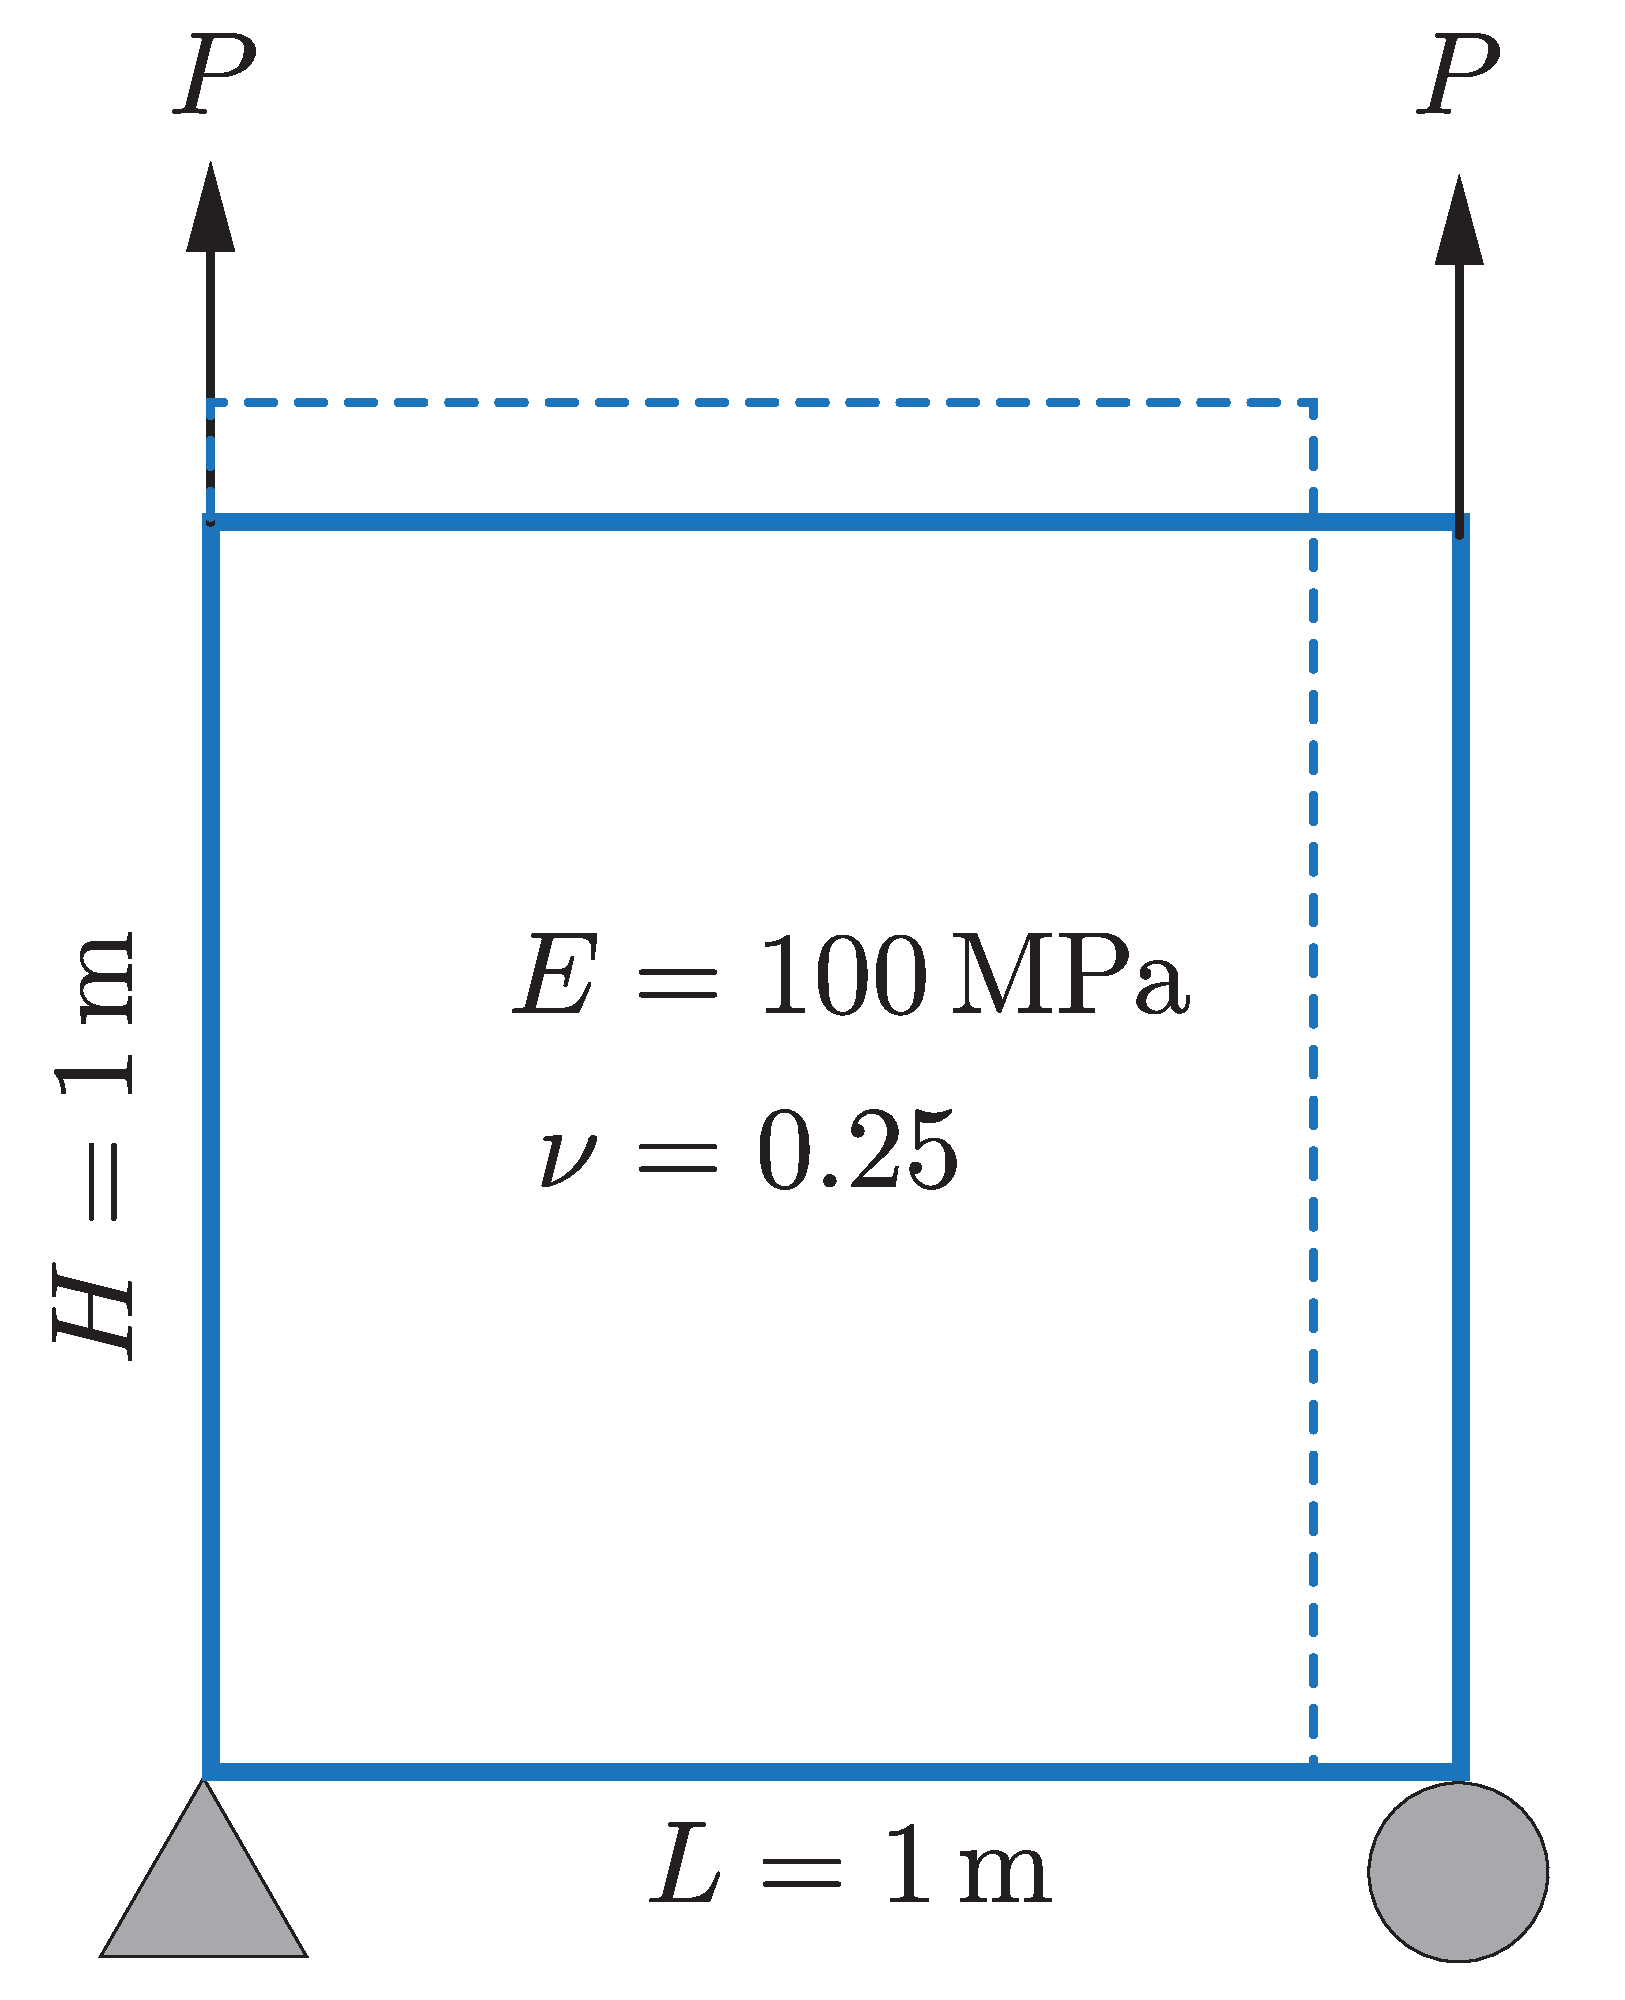
\includegraphics[width=\textwidth]{final/part1/final1_test_setup.pdf}
    \caption{Element mesh and boundary conditions for the uniaxial tension test. $P$ varys from $0$ to $\qty{1e8}{\newton}$. }
\end{subfigure}
\begin{subfigure}{0.55\textwidth}
    \centering
    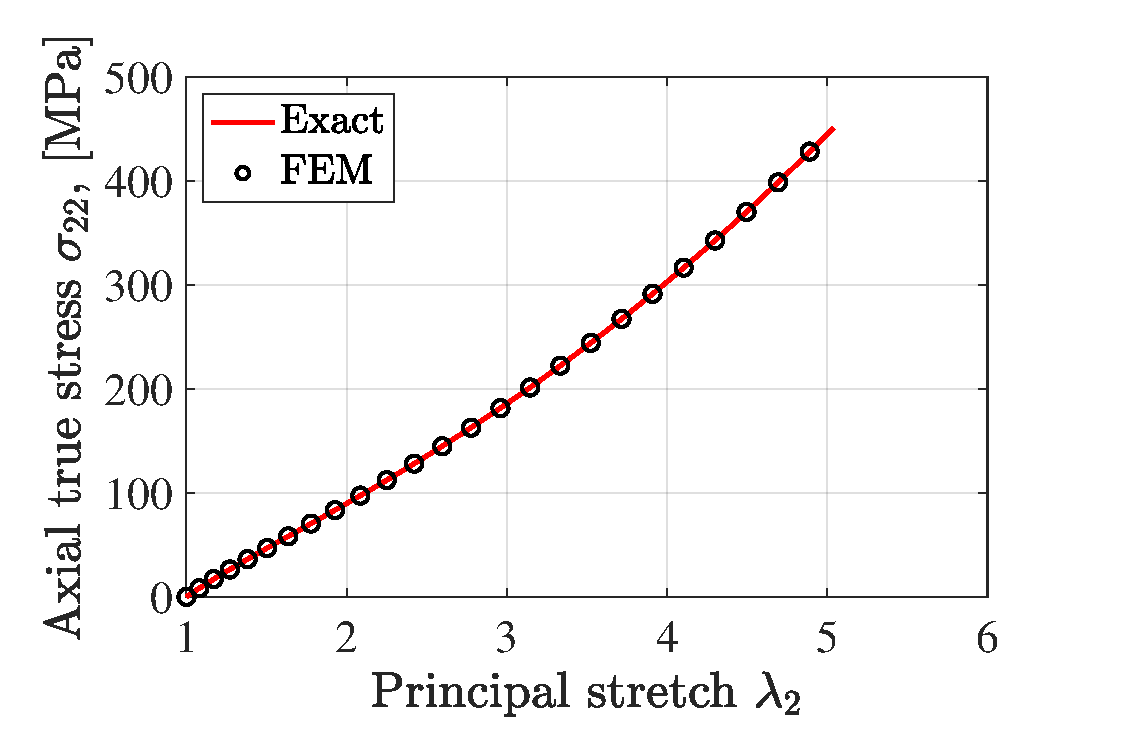
\includegraphics[width=\textwidth]{final/part1/final1_test.pdf}
    \caption{Axial stress as a function of principal strain in the $y$-direction. The black circles are the numerical results with 100 load steps, sampled every 4 steps. The red line is the ``exact'' solution computed via MATLAB \code{fsolve}.}
\end{subfigure}
\caption{Finite element setup and result of the uniaxial tension test. }
\label{fig:final1_test}
\end{figure}

\section{Results}
For the two cases of interests, we assume the following:
\begin{itemize}
    \item Modified Newton-Raphson method is used with a relative tolerance of $10^{-9}$.
    \item All data is tracked at integration point 3 in the given figure, which is integration point 4 in the code (north-west quadrant). 
    \item Material properties $\lambda$ and $\mu$ are computed using linear elasticity. 
\end{itemize}

\begin{table}[!ht]
\centering
\begin{tabular}{|c|c|c|c|c|c|}
    \hline
    Step / Total steps & Iter 0 & Iter 1 & Iter 2 & Iter 3 & Iter 4 \\
    \hline 
    10 / 100 & 1 & 1.3879e-3 & 3.6500e-6 & 9.7155e-9 & 2.58881e-11 \\
    \hline 
    50 / 100 & 1 & 1.3662e-3 & 3.5068e-6 & 9.1435e-9 & 2.3830e-11 \\
    \hline 
    10 / 200 & 1 & 6.9174e-4 & 9.0755e-7 & 1.2046e-9 & 1.2979e-12 \\
    \hline
    50 / 200 & 1 & 6.8776e-4 & 8.9372e-7 & 1.1766e-9 & 1.5088e-12 \\
    \hline
\end{tabular}
\caption{\emph{Case (a)} residual reduction for selected load steps and total steps, denoted in the first column as Step / Total steps. For  example, the first row of data entry represents residual reduction at step 10 for a total of 100 load steps.}
\end{table}

\begin{table}[!ht]
\centering
\begin{tabular}{|c|c|c|c|c|c|}
    \hline
    Step / Total steps & Iter 0 & Iter 1 & Iter 2 & Iter 3 & Iter 4 \\
    \hline 
    10 / 100 & 1 & 1.8786e-3 & 9.4634e-7 & 3.8755e-9 & 2.7572e-12 \\
    \hline 
    50 / 100 & 1 & 1.8743e-3 & 9.4646e-7 & 3.8558e-9 & 2.7073e-11 \\
    \hline 
    10 / 200 & 1 & 9.3464e-4 & 2.3420e-7 & 4.7985e-10 & -- \\
    \hline
    50 / 200 & 1 & 9.3411e-4 & 2.3421e-7 & 4.7717e-10 & -- \\
    \hline
\end{tabular}
\caption{\emph{Case (b)} residual reduction for selected load steps and total steps, denoted in the first column as Step / Total steps. For  example, the first row of data entry represents residual reduction at step 10 for a total of 100 load steps.}
\end{table}

\begin{figure}[!ht]
    \centering
    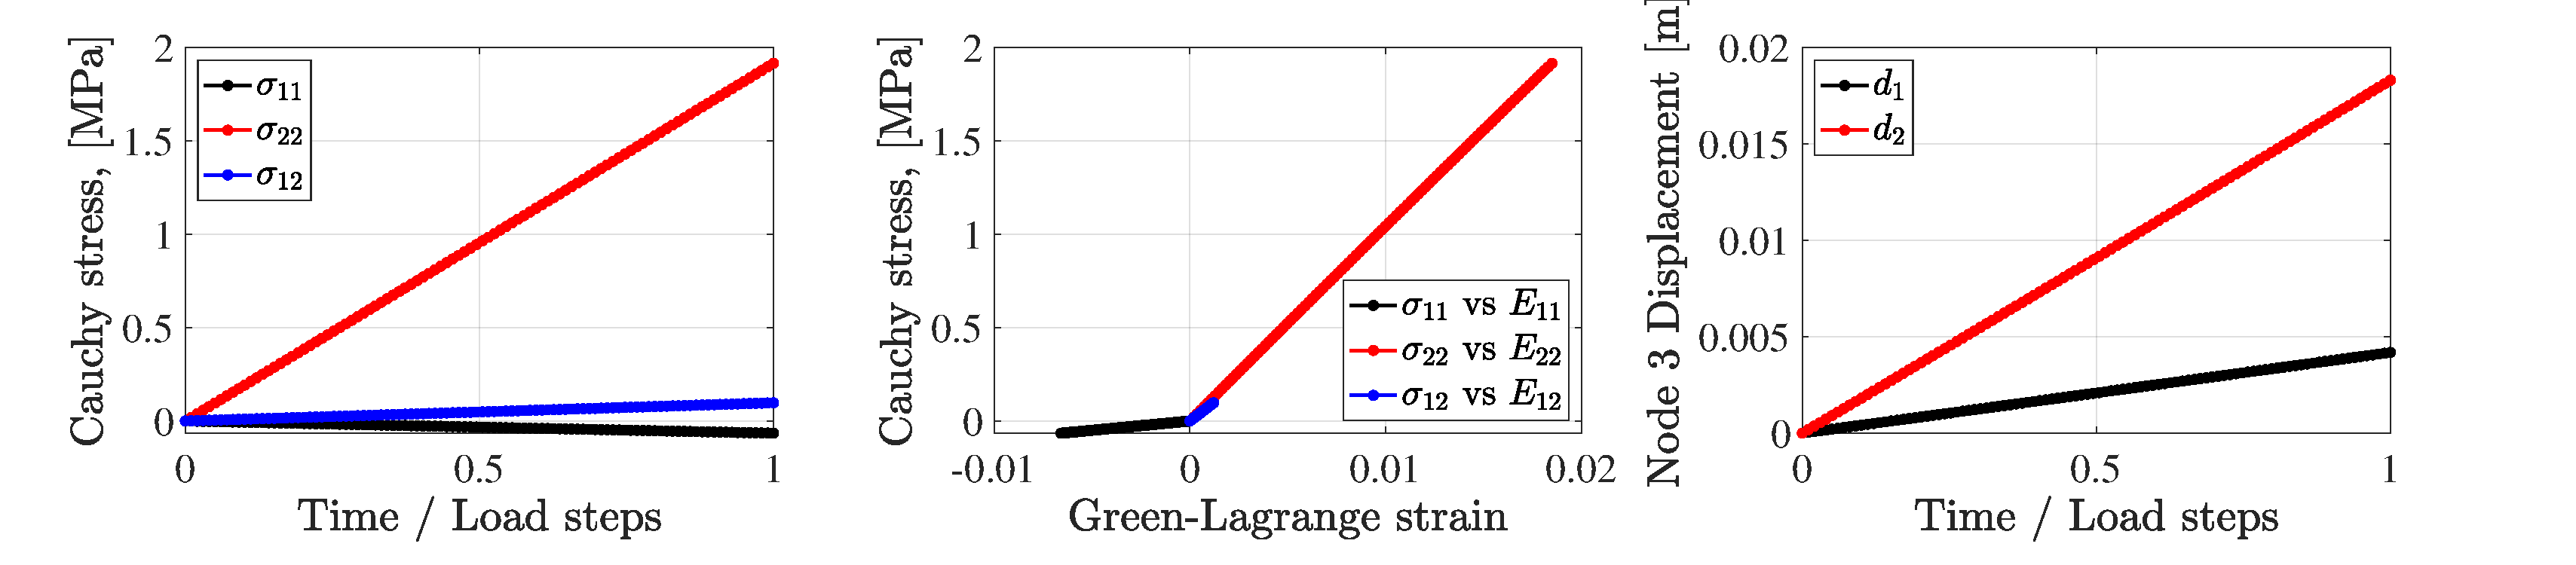
\includegraphics[width=\linewidth]{final/part1/final1_stretch.pdf}
    \caption{Diagnostics regarding case (a). }    
    \label{fig:final1_stretch}
\end{figure}

\begin{figure}[!ht]
    \centering
    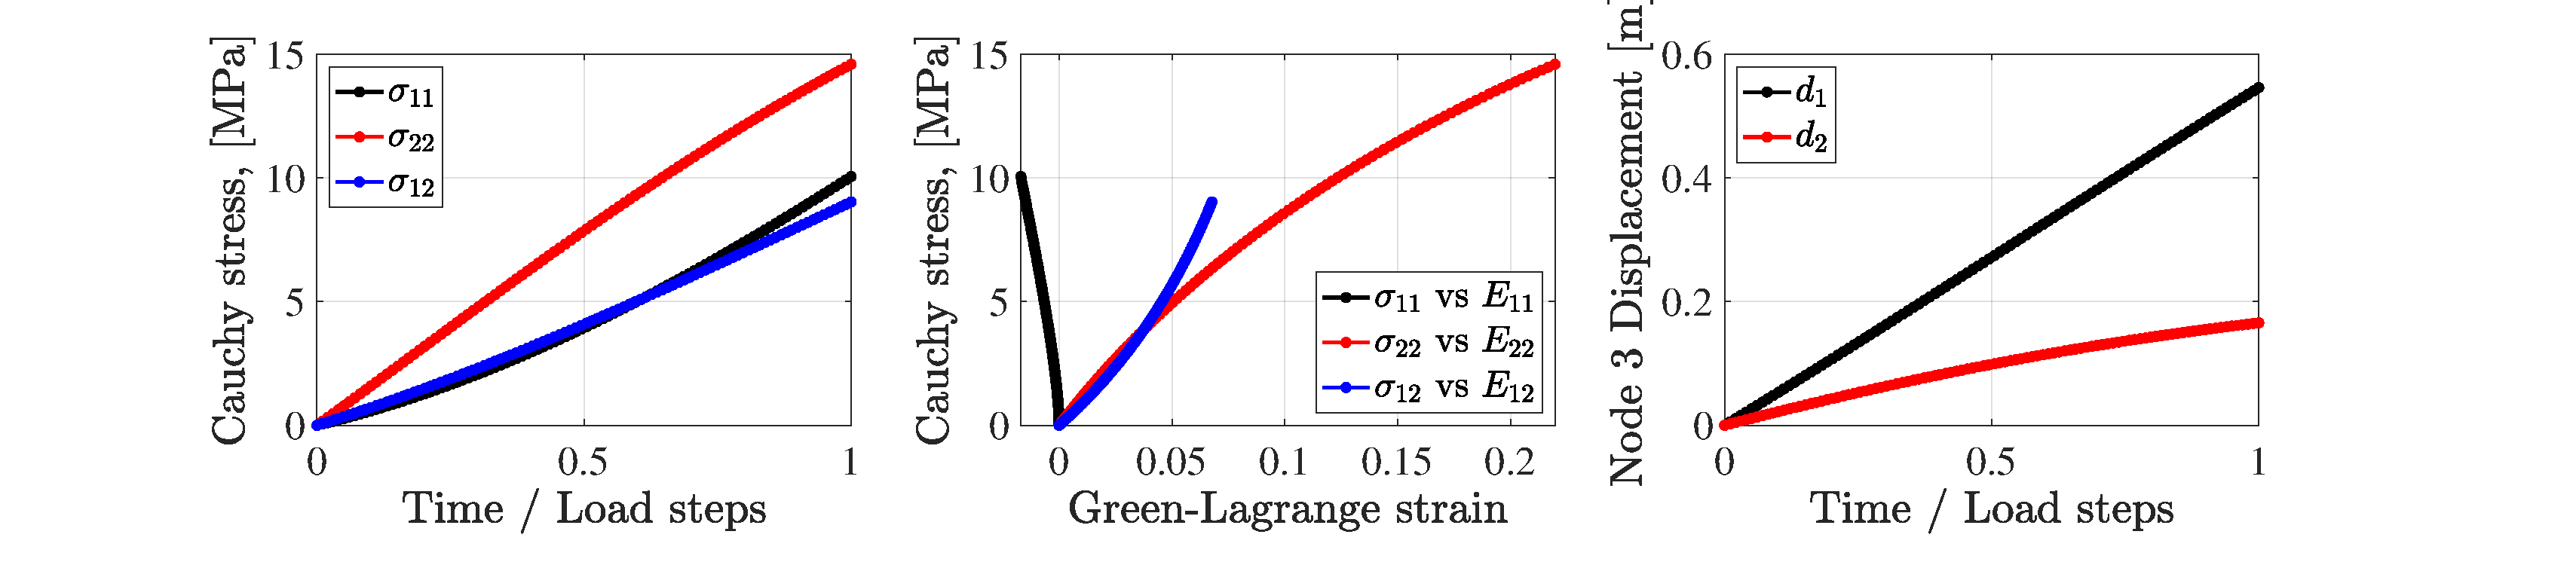
\includegraphics[width=\linewidth]{final/part1/final1_shear.pdf}
    \caption{Diagnostics regarding case (b). }    
    \label{fig:final1_shear}
\end{figure}

\begin{figure}[!ht]
    \centering
    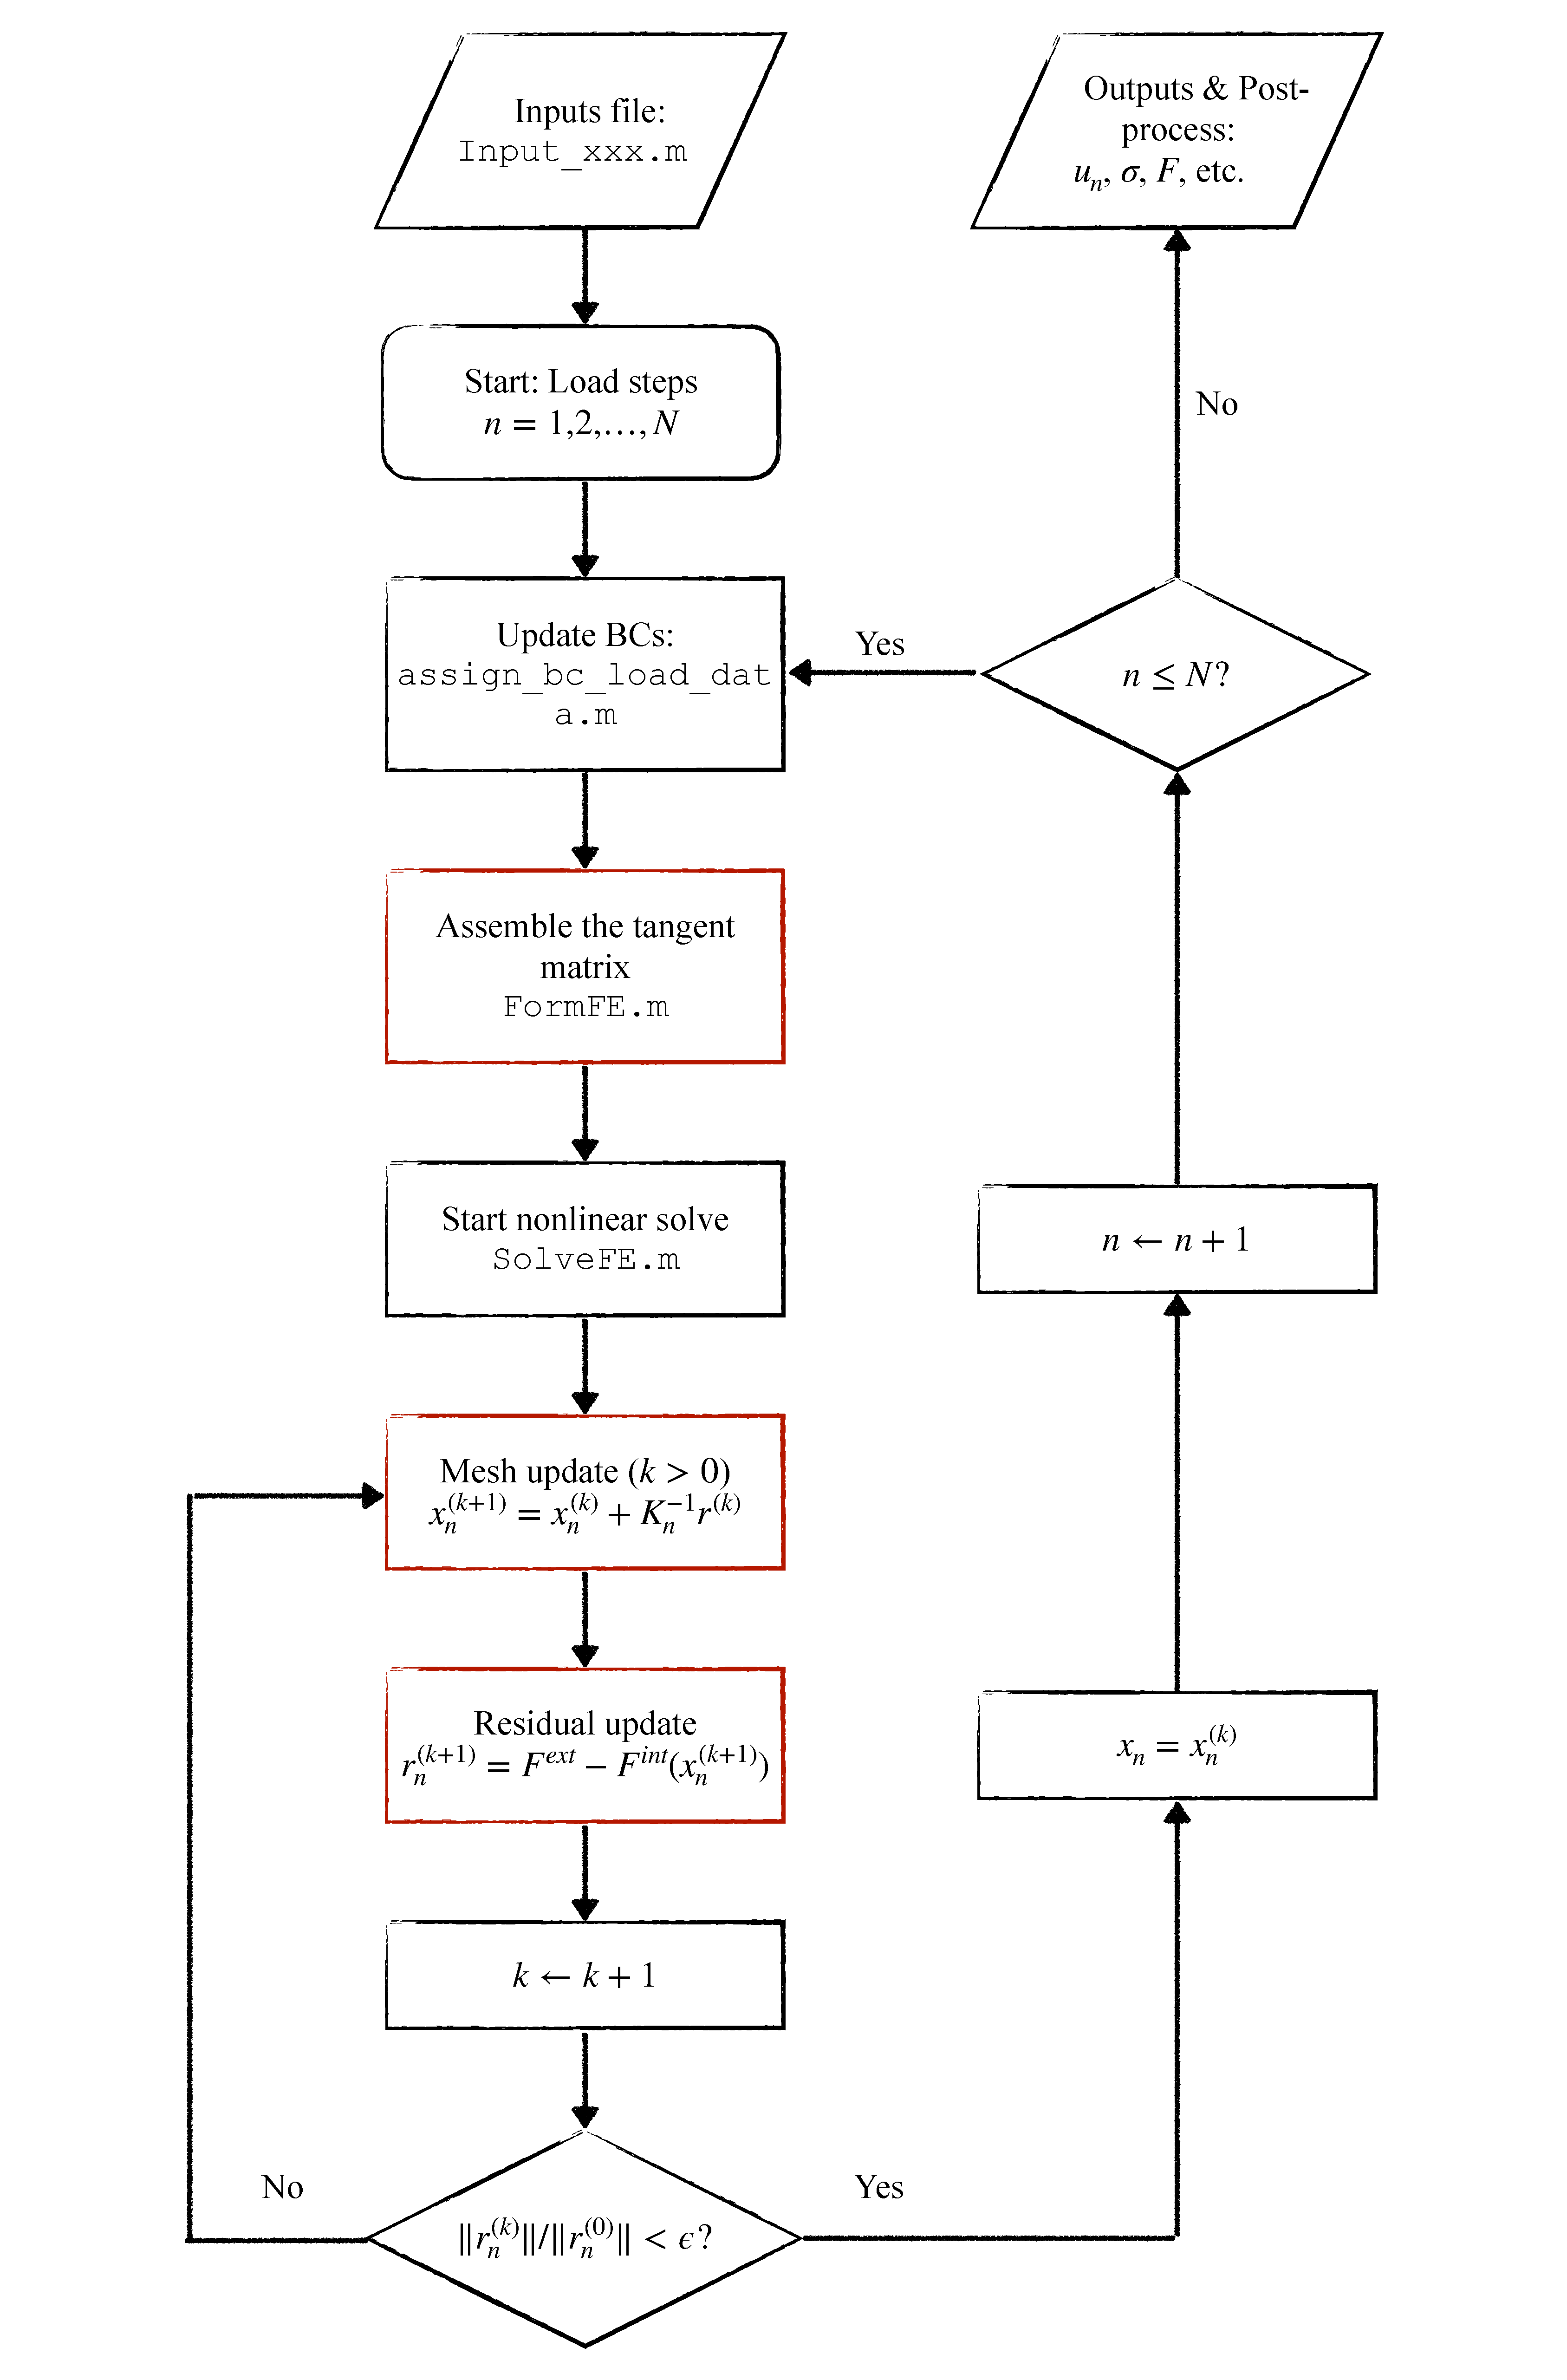
\includegraphics[width=0.9\linewidth]{final/part1/flow_chart_all.pdf}
    \caption{Overall flow chart for solving the nonlinear finite-strain elastostatic problem.}    
    \label{fig:final1_flow_chart_all}
\end{figure}
\begin{figure}[!ht]
    \centering
    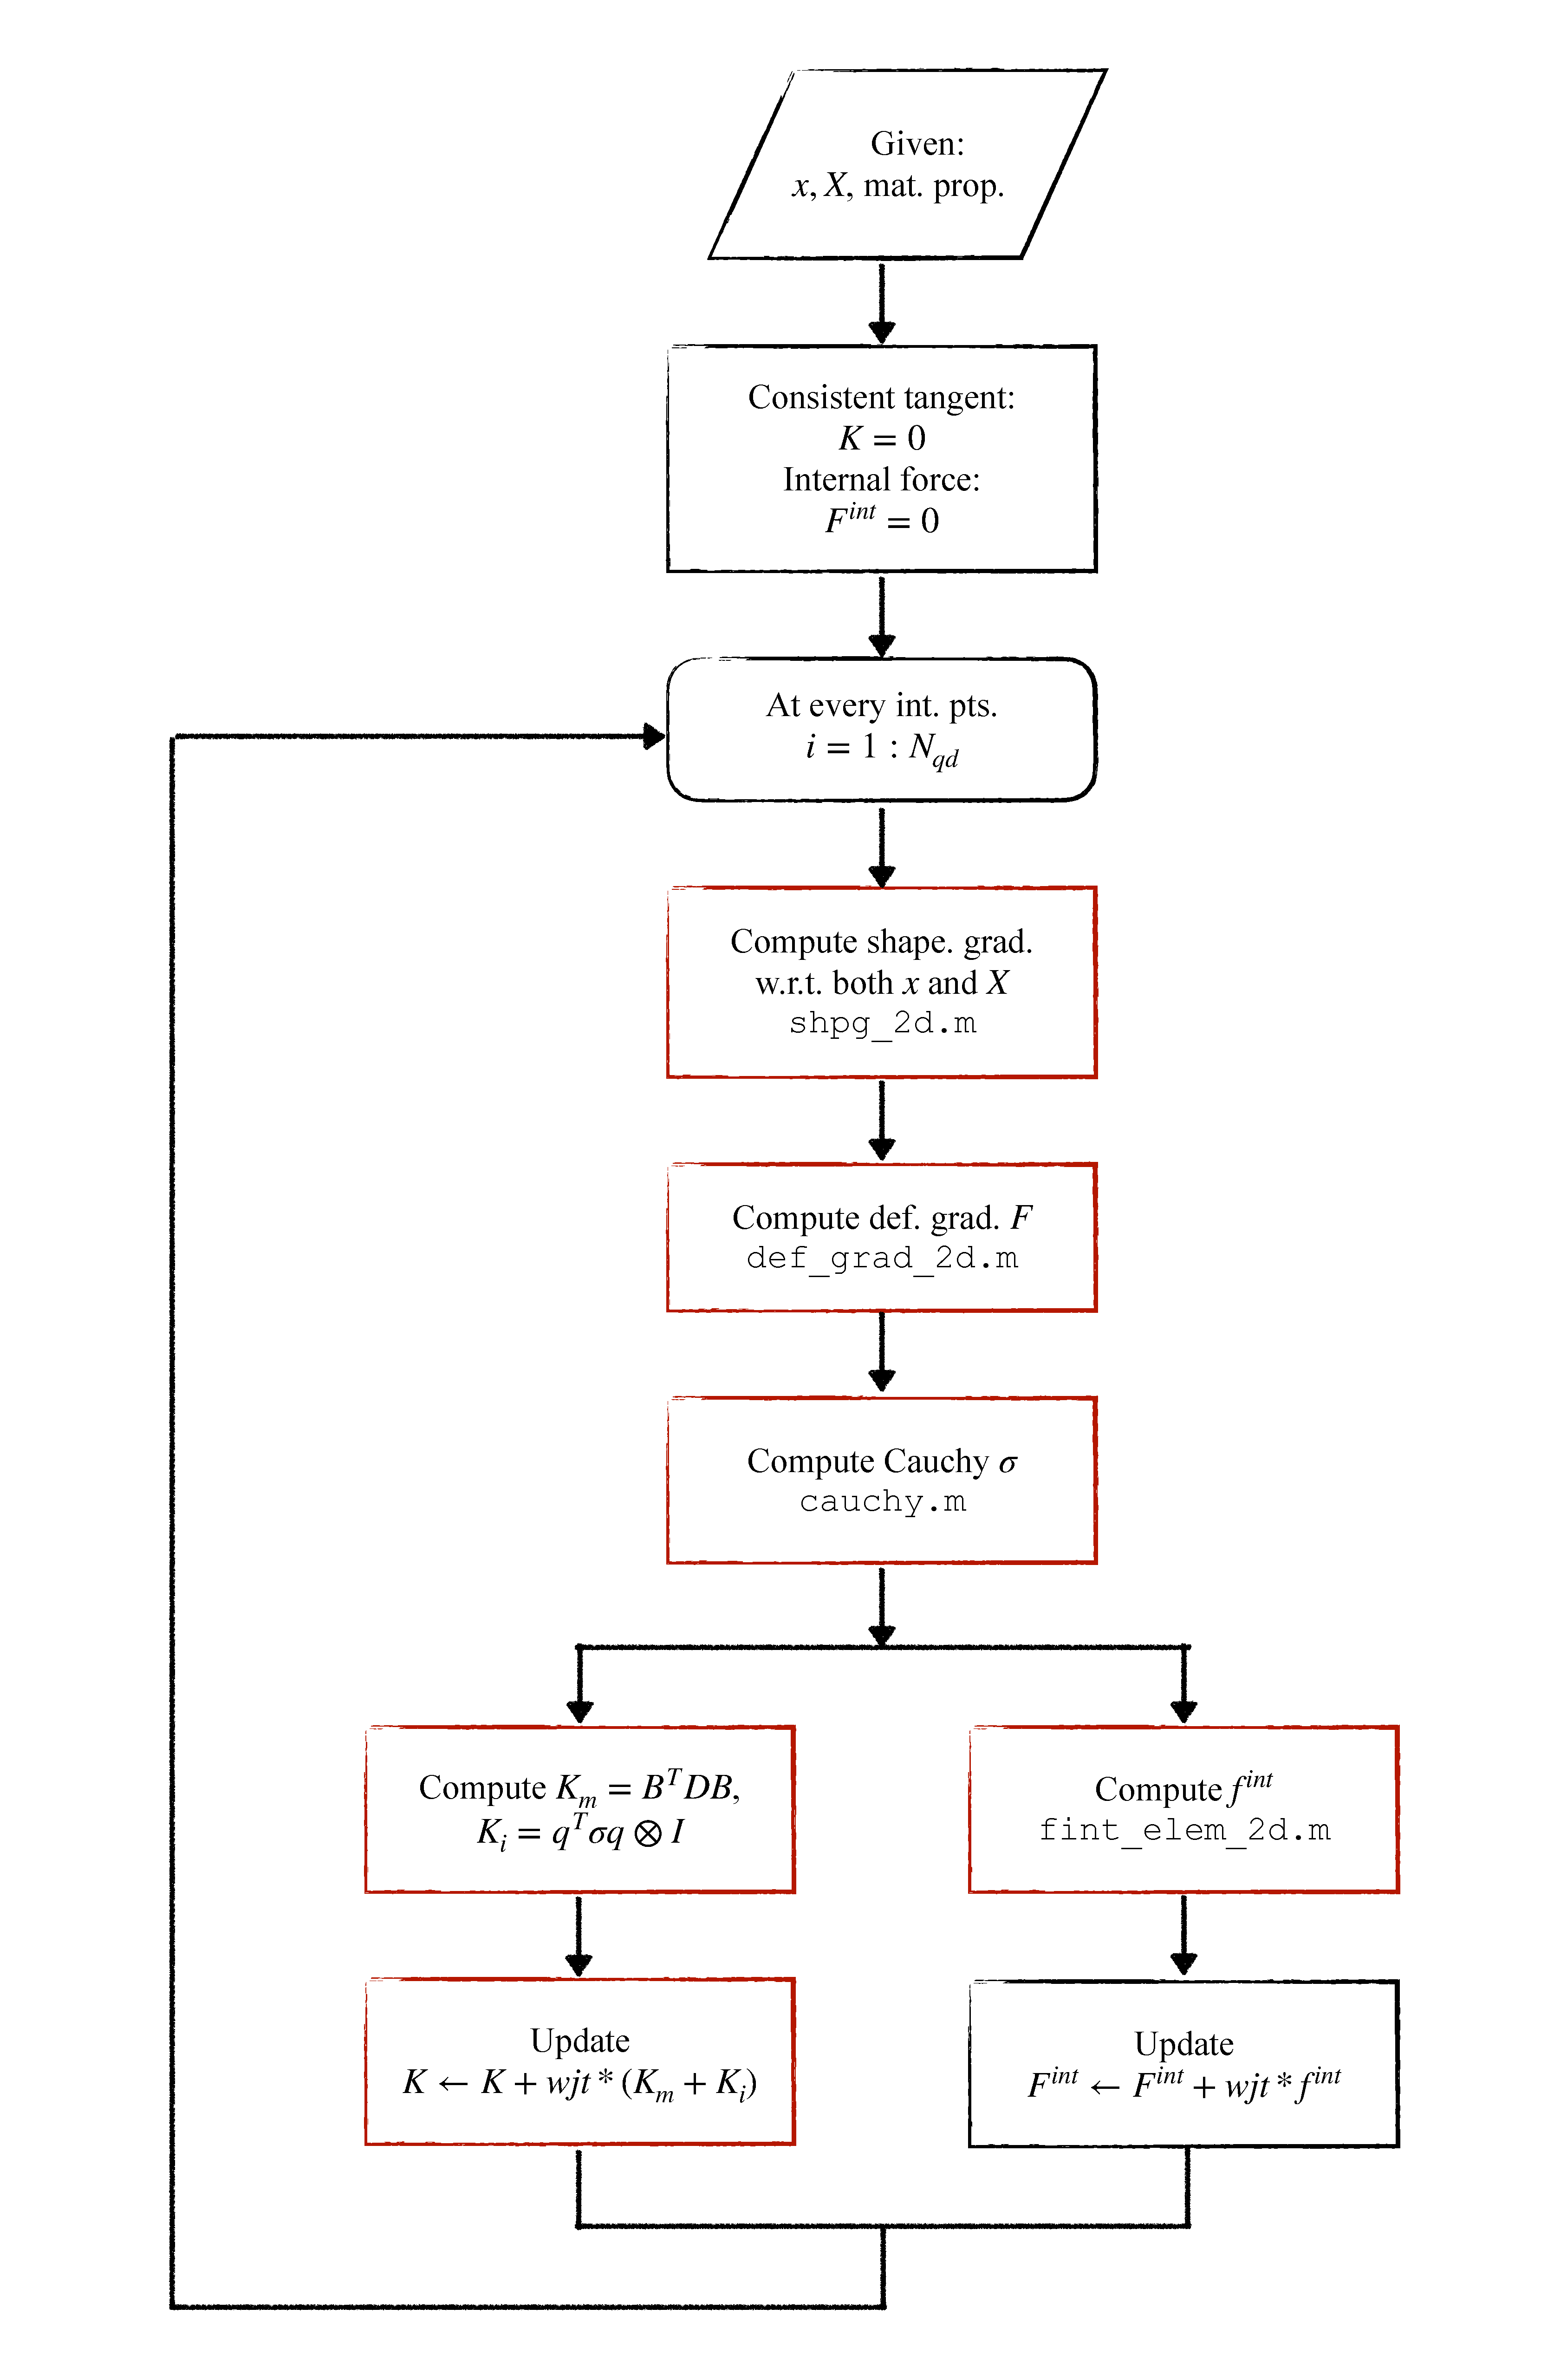
\includegraphics[width=0.85\linewidth]{final/part1/flow_chart_int.pdf}
    \caption{Flow chart for computing the consistent tangent and internal force vector for the hyperelasticity problem.}    
    \label{fig:final1_flow_chart_int}
\end{figure}